%
% File acl2017.tex
%
%% Based on the style files for ACL-2015, with some improvements
%%  taken from the NAACL-2016 style
%% Based on the style files for ACL-2014, which were, in turn,
%% based on ACL-2013, ACL-2012, ACL-2011, ACL-2010, ACL-IJCNLP-2009,
%% EACL-2009, IJCNLP-2008...
%% Based on the style files for EACL 2006 by 
%%e.agirre@ehu.es or Sergi.Balari@uab.es
%% and that of ACL 08 by Joakim Nivre and Noah Smith

\documentclass[11pt,a4paper]{article}
\usepackage[hyperref]{acl2017}
\usepackage{times}
\usepackage{latexsym}

\usepackage{url}

%\aclfinalcopy % Uncomment this line for the final submission
%\def\aclpaperid{***} %  Enter the acl Paper ID here

%\setlength\titlebox{5cm}
% You can expand the titlebox if you need extra space
% to show all the authors. Please do not make the titlebox
% smaller than 5cm (the original size); we will check this
% in the camera-ready version and ask you to change it back.

\newcommand\BibTeX{B{\sc ib}\TeX}

\title{Instructions for ACL-2017 Proceedings}

\author{First Author \\
  Affiliation / Address line 1 \\
  Affiliation / Address line 2 \\
  Affiliation / Address line 3 \\
  {\tt email@domain} \\\And
  Second Author \\
  Affiliation / Address line 1 \\
  Affiliation / Address line 2 \\
  Affiliation / Address line 3 \\
  {\tt email@domain} \\}

\date{}

\begin{document}
\maketitle
\begin{abstract}
  This document contains the instructions for preparing a camera-ready
  manuscript for the proceedings of ACL-2017. The document itself
  conforms to its own specifications, and is therefore an example of
  what your manuscript should look like. These instructions should be
  used for both papers submitted for review and for final versions of
  accepted papers.  Authors are asked to conform to all the directions
  reported in this document.
\end{abstract}

%!TEX root = ../main.tex

In this section, we describe our efforts to create a new, large-scale
linguistics resource: a semantically annotated grammar with wide-coverage of
English, accompanied by a semantically annotated WSJ corpus. This research seeks
to build upon the grammar created for the S-STRUCT experiments in Section
\ref{sec:sstruct_dataset}, which consisted of 30 unlexicalized XTAG trees with
hand-annotated semantics. 

While this grammar was sufficient for the scaling
experiments, it still suffered from a few problems. First, it still does not
have enough coverage of English; only the 30 most frequently used XTAG trees
have semantics, whereas there are over 1000 trees available in the XTAG corpus.
Secondly, the semantics were still ad-hoc in the sense that different predicates
have no similarity measure; either they are the same or they are different. For
example, $run(x)$ and $chase(x,y)$ are different predicates, but both express
some form of motion. In the previously discussed semantics, these are treated as
entirely dissimilar, but ideally we would have some level of abstraction
allowing us to express their similarity. Finally, the current semantic system
cannot represent higher-order semantic concepts such as adverbs, which modify
verbs (predicates).

In this section, we attempt to improve upon all of these shortcomings. We explore the
alternative semantic representations of Davidsonian and Neo-Davidsonian semantics, which
reify verbal predicates with an explicit ``event'' entity. We leverage the existing 
linguistics resources of VerbNet and PropBank to expand our semantic coverage of declarative verb trees in the XTAG grammar. Finally,
we use ideas from grammar metarules and metagrammars to increase our semantic coverage of XTAG verb trees by an order of magnitude. The end result of this process is a higher-quality semantically annotated grammar with vastly wider
coverage. We then show the utility of this grammar by using it to create a semantically annotated version of the WSJ corpus.

%The motivation for this section is
%asking ``can we expand upon the coverage and expressibility of this grammar 
%to provide a resource that the rest of the linguistics community will
%find useful?'' In the remainder of this section, we provide the necessary linguistics 
%background and describe the contributions we have made in this area.

\section{Background}

Before discussing our linguistic resource, we must review some 
linguistics background. In this section, we consider alternative semantic 
representations to those used in Section \ref{sec:lambda_semantics}. We then
explore existing linguistics resources, VerbNet and PropBank, to see if we can 
leverage existing work. Finally we investigate automated ways of expanding 
grammar coverage through metagrammars and metarules.

\subsection{Davidsonian and Neo-Davidsonian Semantics}
\label{sec:neodavidsonian}

In Section \ref{sec:lambda_semantics}, we introduced a first-order logical
semantic  representation, augmented with $\lambda$-calculus notation to allow
for compositionality. In this representation, variables represent entities in
the world  (with either existential or universal quantification) and predicates
represent the relations between entities in the world. We will refer to these
semantics as ``Classical Semantics'', to maintain convention with
\cite{neodavidsonian}. If we wanted to represent the semantics for the
transitive verb ``chase'', we would  write:

\begin{align}
chase.semantics \coloneqq \lambda x \lambda y \left[ chase(x,y) \right] && \text{Classical}
\end{align}

In his 1967 seminal work, Donald Davidson argues that predicates
representing actions (syntactically, this means verbs) require an additional
``event'' argument that classical semantics do not include
\cite{davidson1967logical}. Consider the following piece of text: ``Jones did it
with a knife. What he did was butter a piece of toast.'' Davidson argues that
in this piece of text, ``it'' appears to refer to some entity, presumably an
action. If we wanted to characterize the semantics of the first sentence, we may
write something conveying ``there is an action $x$ such that Jones did $x$ with a
knife'' \cite{davidson1967logical}. However, when we try to substitute something
for $x$, there is no suitable candidate, as variables are representing
entities.

Additionally, if we were to write the sentence ``Jones buttered a piece of toast
with a knife'',  we would expect the same semantic representation as the first
piece of text. However, in the classical representation of $buttered(Jones, t,
k) \land toast(t) \land knife(k)$, we would no longer see the $x$ variable that
we had observed in the first representation. Because of this phenomenon (and
many other phenomena which Davidson discusses in \cite{davidson1967logical}),
Davidson argues that predicates representing actions require a special event
variable. We refer to this formalism as ``Davidsonian Semantics''. From this
perspective, we could rewrite the semantics for $chase$ as:

\begin{align}
chase.semantics \coloneqq \lambda x \lambda y \left[ chase(e,x,y) \right] && \text{Davidsonian}
\end{align}

This would allow us to represent both toast-buttering examples with semantics
such as: $buttered(e, Jones, t, k) \land toast(t) \land knife(k)$.

While this solves the problems in the previous example, it raises additional
questions as well. What if our sentence were ``Jones buttered a piece of toast
slowly with a knife in the kitchen''? Do we represent $buttered$ as a 6-tuple
where all of these pieces of information are arguments? What if one is missing?
If we add ``at Midnight'' to the sentence, do we  create a new predicate taking
7 arguments?

These questions have led to a further semantic representation, called ``Neo-Davidsonian'' semantics. In both classical and Davidsonian semantics, entities
derive their relationship with an action from their index in the argument list.
When we write $chase(x,y)$ we know that $x$ is the subject (the entity doing the
chasing) and $y$ is the object (the entity being chased) because of their
argument index. In Neo-Davidsonian semantics, entities are related to actions by {\em thematic indexing} instead. An action is represented as a predicate taking only an event variable as an argument; then, special predicates called {\em thematic roles}
are used to assign entities their relationship to the event variable
\cite{neodavidsonian}. These thematic roles can be broad roles that apply to
many actions, such as $Agent$ and $Theme$, or narrow roles that are specific to
the action, such as $chaser$ and $chasee$ \cite{baker1997thematic}. We will
assume broad roles in our work. In Neo-Davidsonian Semantics, we would rewrite
our $chase$ semantics as:

\begin{align}
chase.semantics \coloneqq \lambda x \lambda y \left[ chase(e) \land Agent(e,x) \land Theme(e, y) \right] && \text{Neo-Davidsonian}
\end{align}

While this formalism is theoretically equivalent to Davidsonian semantics
\cite{neodavidsonian}, the flexibility of the representation allows for
intuitive solutions to missing or extra arguments. Looking back at our toast-buttering 
example, we could represent ``Jones buttered a piece of toast slowly
with a knife in the kitchen'' as:

\begin{align*}
& buttered(e) \land Agent(e,Jones) \land Theme(e,t) \\
& \land toast(t) \land slowly(e) \land Location(e,k1) \\
& \land kitchen(k1) \land Instrument(e, k2) \land knife(k2)
\end{align*}

\subsection{VerbNet}

VerbNet is a hierarchical, broad-coverage verb lexicon for English
\cite{verbnet}, in which verbs are organized into verb classes. The verb classes
are derived from Levin classes, an approach to verb classification in which the
verb classes are defined by the set of legal syntactic transformations (called
diathesis alternations) that the verbs can undergo \cite{levin1993english}. For
example, the $Break$ verb class contains verbs such as: $break$, $chip$,
$crack$, $crush$, $fracture$, $rip$, $smash$, $snap$, etc. These can be used
transitively (``John broke the window''), intransitively (``The window broke''),
and in middle constructions (``Glass breaks easily''). Many verbs are present in
multiple Levin classes, giving them a wide range of semantic possibilities
\cite{verbnet}. To account for this in VerbNet, the Levin classes were augmented
with $intersective$ verb classes, which makes a new verb class from each of the
different intersections formed by the original verb classes.

\begin{figure}[h]
\begin{centering}
    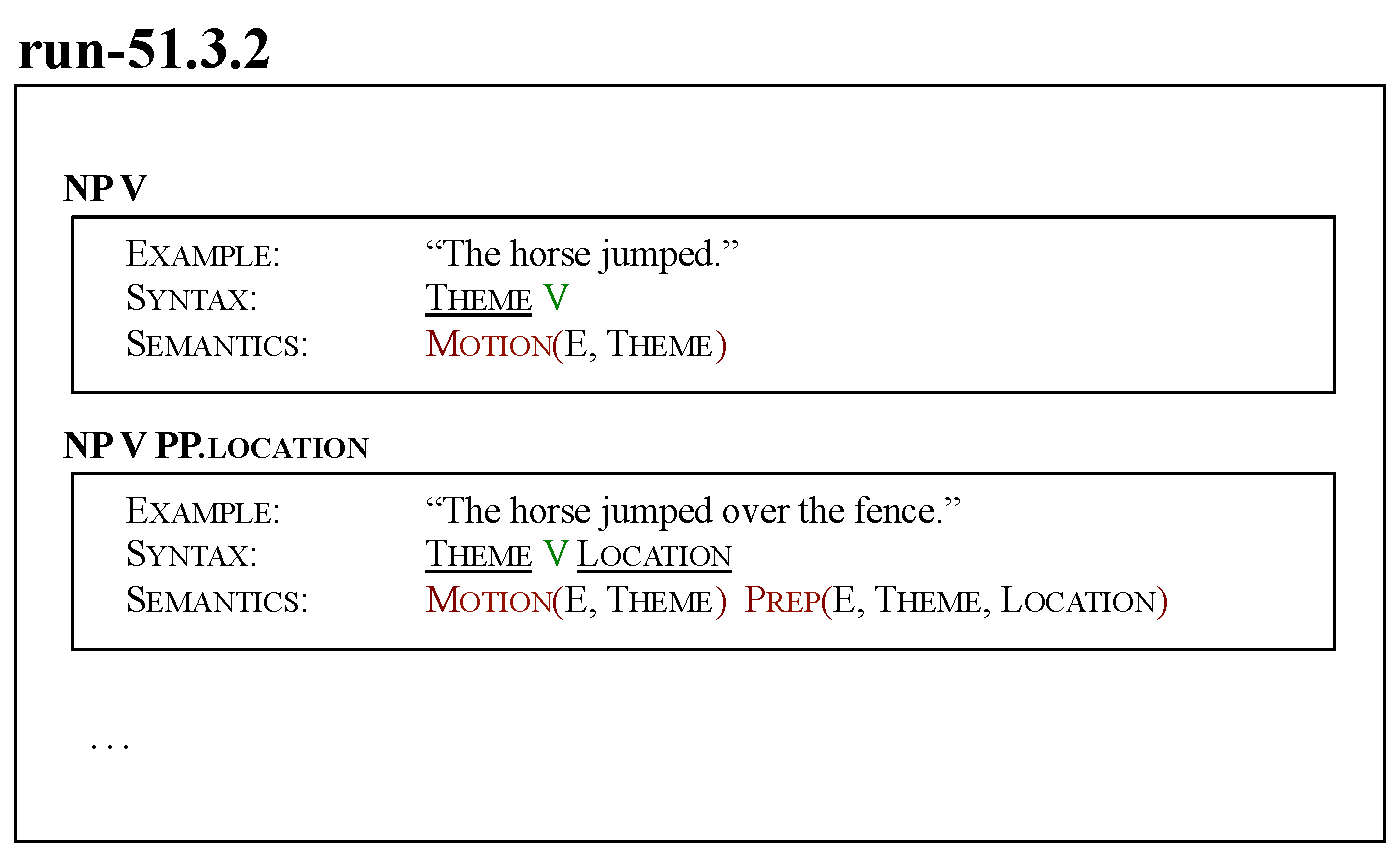
\includegraphics[width= \linewidth ]{resources/ch5_resources/verbnet_frame.pdf}
    \caption{VerbNet class $run\text{-}51.3.2$ with two example frames shown}
    \label{fig:verbnet}
\end{centering}
\end{figure}

Each VerbNet class consists of a set of syntactic frames, which are the
diathesis alternations available to the verbs in the class (transitive,
intransitive, ditransitive, etc). Each frame consists of a usage example, a
syntactic representation, and a semantic representation supporting both Davidsonian and Neo-Davidsonian semantics and
using broad thematic roles \cite{verbnet}. Additionally, the thematic roles can
have semantic restrictions (such as $animate$, $human$, $organization$) that
limit the types of entities that can fill the role. Figure \ref{fig:verbnet}
shows two frames from the $run\text{-}51.3.2$ VerbNet class, which contains
verbs such as $run$, $jump$, $climb$. The first frame shows a typical intransitive
alternation. The semantics tell us that there is an event in which a $Theme$
entity is in motion. The second frame includes a preposition, which adds
a $Location$ role after the verb. The semantics tell us that, not only is there 
an event in which a $Theme$ entity is in motion, but also that the $Theme$ entity's
motion has a specific spatial relationship with a $Location$ entity. 
When this frame is used, a specific preposition would be filled in for $Prep$, 
telling us whether the $Theme$ is moving $over$, $under$, $around$, etc the 
$Location$.

\begin{figure}[h]
\begin{centering}
    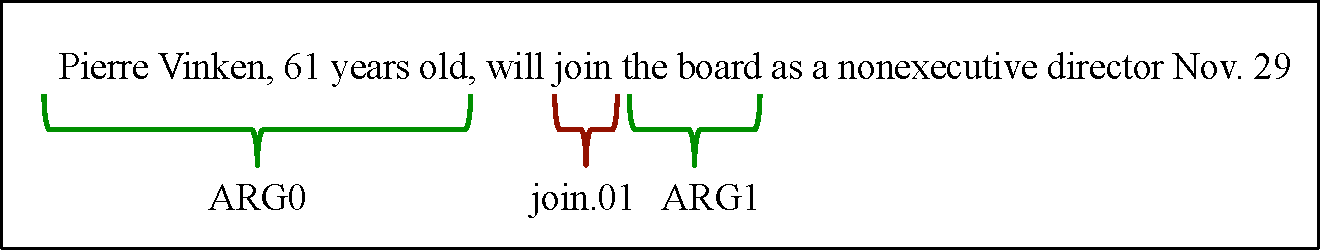
\includegraphics[width=1.0 \linewidth ]{resources/ch5_resources/propbank.pdf}
    \caption{Example PropBank annotation of first WSJ sentence. $join.01$ is a verb template with word span arguments shown.}
    \label{fig:propbank}
\end{centering}
\end{figure}

A major benefit of the VerbNet corpus is that it has been mapped to other
linguistics resources \cite{verbnet}. One such resource is PropBank, a template-based annotation of the Penn TreeBank \cite{propbank}. Every verb is marked with
a template indicating the verb-sense, and specific word-spans are annotated as
arguments to the verb. Figure \ref{fig:propbank} shows an example PropBank
annotation. $join.01$ is a verb template corresponding to the VerbNet class
$mix\text{-}22.1\text{-}2$. The ARG0 and ARG1 word spans serve as the subject and
object of the $join.01$ template.

In addition to PropBank, VerbNet also has mappings to XTAG. In
\cite{ryant2004assigning}, each VerbNet frame, as identified by a ``primary''
and ``secondary'' label, is associated with an XTAG tree family. There are 196
unique frames in VerbNet, and a mapping is identified for all but 18 of these.
Figure \ref{fig:vnet_xtag_mapping} shows the declarative trees for the tree
families corresponding to the frames in Figure \ref{fig:verbnet}.

\begin{figure*}[h]
    \centering
    \begin{subfigure}{0.36\textwidth}
        \centering
        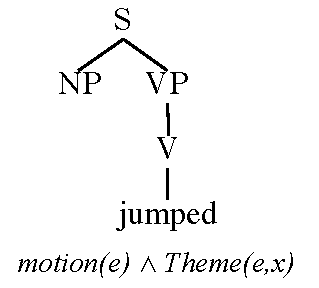
\includegraphics[width=1.0 \linewidth ]{resources/ch5_resources/jump_intransitive.pdf}
        \caption{$\alpha nx0V$}
        \label{fig:jump_intransitive}
    \end{subfigure}
    \begin{subfigure}{0.4\textwidth}
        \centering
        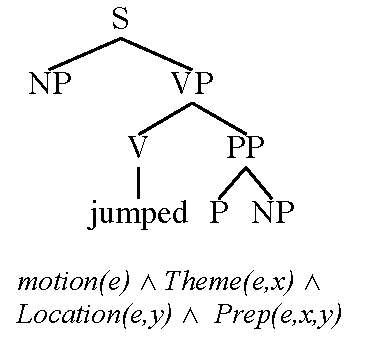
\includegraphics[width=1.0 \linewidth ]{resources/ch5_resources/jump_intransitive_pp.pdf}
        \caption{$\alpha nx0Vpnx1$}
        \label{fig:jump_intransitive_pp}
    \end{subfigure}
    \centering
    \caption{Declarative trees from XTAG tree families corresponding to \textbf{NP V} and \textbf{NP V PP} VerbNet frames, respectively.}
    \label{fig:vnet_xtag_mapping}
\end{figure*}

\subsection{Metarules and Metagrammars}
\label{sec:metarules}

One disadvantage of a large-scale grammar such as XTAG is that the large number
of trees makes it difficult to add new information. If we decide to add a new 
feature to the grammar (semantic or otherwise), there are $>1000$ trees that 
would have to be manually updated to support this feature \cite{xtag}. One 
strategy to alleviate this problem is to find a more compact representation
for the grammar. Of the $1004$ elementary trees in XTAG, 783 are for verbs 
\cite{prolo2002generating}. These verb trees are already organized into ``tree 
families'' as discussed in Section \ref{sec:pltag}, which consist of a standard, 
declarative tree and then many syntactic variants of the declarative tree. This
structure indicates that a compact abstraction is likely possible. Two separate, 
but related, strategies have been applied to form this abstraction: metarules 
and metagrammars. 

\begin{figure}[h]
\begin{centering}
    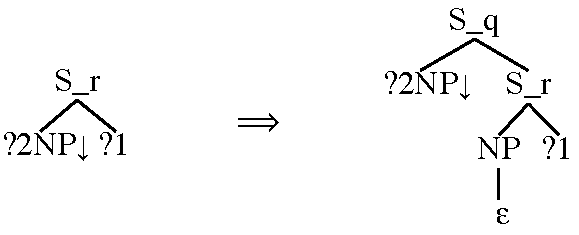
\includegraphics[width=.7 \linewidth ]{resources/ch5_resources/metarule.pdf}
    \caption{Metarule for wh-movement of subject}
    \label{fig:metarule}
\end{centering}
\end{figure}

Becker \cite{becker1994patterns,becker2000patterns} proposed the idea that a
grammar is the closure of the set of base trees under metarule application.  He
identifies 21 rules that allow for transformations such as passives, gerunds,
PRO subjects, wh-movement, imperatives, and relative clauses. Metarules are
encoded with a partial tree on the left-hand side (LHS) and right-hand side
(RHS). When the partial tree on the LHS  matches the structure of a declarative
tree (potentially using wildcards), the metarule can be applied. The RHS
specifies a transformation of the nodes in the LHS, and may introduce additional
nodes as well. Figure \ref{fig:metarule} shows the metarule for wh-movement
of the subject in a declarative tree. The LHS tells us that we can
apply this rule to any tree with an $S$ start symbol that has two children: the
left child must be an $NP$ and the right child can be anything. The RHS tells us
how to transform the input tree: The $NP$ child (representing the subject) gets
extracted, leaving a trace $NP$ as the sibling of the right child. An example
application of this metarule is shown in Figure \ref{fig:metarule_application}.

\begin{figure*}[h]
    \centering
    \begin{subfigure}{0.3\textwidth}
        \centering
        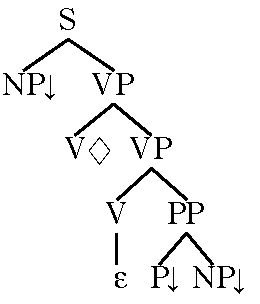
\includegraphics[width=1.0 \linewidth ]{resources/ch5_resources/metarule_declarative.pdf}
        \caption{declarative tree: $\alpha nx0Vpnx1$}
        \label{fig:metarule_declarative}
    \end{subfigure}
    \hfill
    \begin{subfigure}{0.38\textwidth}
        \centering
        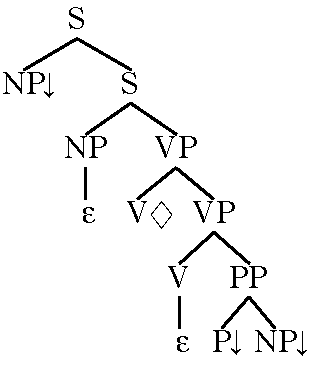
\includegraphics[width=1.0 \linewidth ]{resources/ch5_resources/metarule_subject_extracted.pdf}
        \caption{wh-movement of subject: $\alpha W0nx0Vpnx1$}
        \label{fig:metarule_subject_extracted}
    \end{subfigure}
    \hfill
    \centering
    \caption{Declarative tree undergoing metarule application of metarule in Figure \ref{fig:metarule}, resulting in wh-movement of the subject.}
    \label{fig:metarule_application}
\end{figure*}

Further work by Prolo \cite{prolo2002generating} provided an ordering of the 21
metarules defined by Becker, as shown in Table \ref{tab:metarules}. In this work, the goal was to generate the full set
of XTAG verb trees from the application of metarules to the declarative (base)
trees. To generate trees, metarules were applied to the declarative trees
cumulatively in the defined order. Starting from just the declarative trees, the
first rule was applied; this generated new trees which were included in the
generated set.  These trees, in addition to the previous trees, were passed to
the next metarule, continuing until no metarules remained. In applying this
procedure, 1200 trees were generated \cite{prolo2002generating}. This procedure
failed to generate 20 idiosyncratic  trees and overgenerated 200 trees due to
lexical restrictions on transformations that were unaccounted for. However, on
the whole, this procedure was effective.

\begin{table}[h!]
\centering
\begin{tabular}{|l|l|}
\hline
\textbf{Metarule}       & \textbf{Description}                                                                                                \\ \hline
passive                 & Generate the passive form                                                                                           \\ \hline
passive from PP         & \begin{tabular}[c]{@{}l@{}}Passive form for PP complements: \\ ``Results were accounted for by ...''\end{tabular}   \\ \hline
dropby                  & ``Passive without by-clause''                                                                                       \\ \hline
gerund                  & \begin{tabular}[c]{@{}l@{}}Trees for NPs like ``eating'' in:\\  ``John eating cake (is unbelievable)''\end{tabular} \\ \hline
imperative              & Imperative                                                                                                          \\ \hline
wh-subj                 & Wh-subject movement                                                                                                 \\ \hline
wh-sentsubj             & \begin{tabular}[c]{@{}l@{}}Wh-subject movement for\\ sentential subjects\end{tabular}                               \\ \hline
wh-npobj                & NP extraction from inside objects                                                                                   \\ \hline
wh-smallnpobj           & NP obj. extr. for small clauses                                                                                     \\ \hline
wh-apobj                & AP complement extraction                                                                                            \\ \hline
wh-advobj               & ADVP complement extraction                                                                                          \\ \hline
wh-ppobj                & PP complement extraction                                                                                            \\ \hline
rel-adj-W               & Adjunct relative clause with wh-NP                                                                                  \\ \hline
rel-adj-noW             & \begin{tabular}[c]{@{}l@{}}Adjunct relative clause \\ with complement\end{tabular}                                  \\ \hline
rel-subj-W              & Subject rel. clause with wh-NP                                                                                      \\ \hline
rel-subj-noW            & \begin{tabular}[c]{@{}l@{}}Subject relative clause \\ with complement\end{tabular}                                  \\ \hline
rel-subj-noW-forpassive & \begin{tabular}[c]{@{}l@{}}Subject relative clause with \\ complement for passives\end{tabular}                     \\ \hline
rel-obj-W               & \begin{tabular}[c]{@{}l@{}}NP Object relative clause \\ with wh-NP\end{tabular}                                     \\ \hline
rel-obj-noW             & \begin{tabular}[c]{@{}l@{}}NP Object relative clause \\ with complement\end{tabular}                                \\ \hline
rel-ppobj               & PP Object relative clause                                                                                           \\ \hline
PRO                     & PRO Subject                                                                                                         \\ \hline
\end{tabular}
\caption{Ordered list of metarule transformations}
\label{tab:metarules}
\end{table}

Similar work was done by Alahverdzhieva with {\em XMG} (eXtensible MetaGrammar),
the metagrammar writing environment \cite{alahverdzhieva2008xtag}.  In this
work, the XTAG trees were factorized into a 4-level hierarchy of common
substructures:  tree families, diathesis alternations, syntactic function
classes, and tree fragments. These fragments, along with a set of rules
specifying how these fragments can be combined, enable the generation of larger
trees. The tree fragments and rules were input into the XMG system, which
``compiles'' the metagrammar to produce the full grammar. The output grammar had
full coverage of the XTAG grammar \cite{alahverdzhieva2008xtag}.

\section{Building the Grammar}

In this section we describe the new linguistics resources that we have contributed: 
a semantically annotated grammar with wide-coverage of English, and a semantic annotation of
the WSJ corpus that was derived from the semantic grammar. 

We start with the XTAG grammar, as it already has wide {\em syntactic} coverage 
of English. Additionally, through the XTAG-VerbNet mapping done in \cite{ryant2004assigning},
the most salient tree families have already been given Neo-Davidsonian semantics
by virtue of the mapping to VerbNet frames (which contain these semantic annotations). 

We build on this work in two ways:

\begin{enumerate}

    \item Taking ideas from the metarule and metagrammar research in Section \ref{sec:metarules}, we seek to expand the coverage from the XTAG-VerbNet research by adding semantic rules which correspond to the syntactic tree transformations (passives, wh-movement, etc). Due to the tree family structure and the XTAG naming scheme, we know the base tree and transformations for any verb subcategorization tree in XTAG. By creating semantic rules for these transformations, we can increase our coverage by at least an order of magnitude, as some tree families have over 50 transformations.

    \item Although the verb trees introduce the majority of the semantic content, we still require semantic annotations for the ``individual trees''which represent nouns, adjectives, adverbs, conjunctions, punctuation, etc. so that we can generate full sentences. We provide these annotations by hand, prioritizing trees based on the frequency with which they appear in parses of the WSJ corpus.

\end{enumerate}

\subsection{Mapping an explicit syntax/semantics interface}

The starting place for our semantic annotation of XTAG is the set of semantically annotated base trees given by the VerbNet mapping, as shown in Figure \ref{fig:vnet_xtag_mapping} and Figure \ref{fig:verbnet}. Intuitively, we want to take each expression in the flat semantic representation given by VerbNet and associate it with its corresponding syntactic subtree. Additionally, we want to associate each variable in the semantic expression with its corresponding subtree. For example, in Figure \ref{fig:vnet_xtag_mapping} the NP node should be annotated with the semantic predicate of $Theme(e, x)$ and the entity variable $x$, as it acts as the subject of the sentence. To establish this mapping, we use the following mapping rules: 

\begin{enumerate}

\item The root is annotated with an existentially quantified event variable 
\item The verbal anchor is associated with the verbal predicates ($motion(e)$ in Figure \ref{fig:vnet_xtag_mapping})
\item Nodes representing verbal arguments are annotated with their thematic-role predicates and entity variables ($Theme(e,x)$, $Agent(e, y)$)
\item Prepositional anchors (such as in Figure \ref{fig:jump_intransitive_pp}) receive prepositional predicates ($over(e,x)$, $around(e,y)$)
\end{enumerate}

\begin{figure}[h]
\begin{centering}
    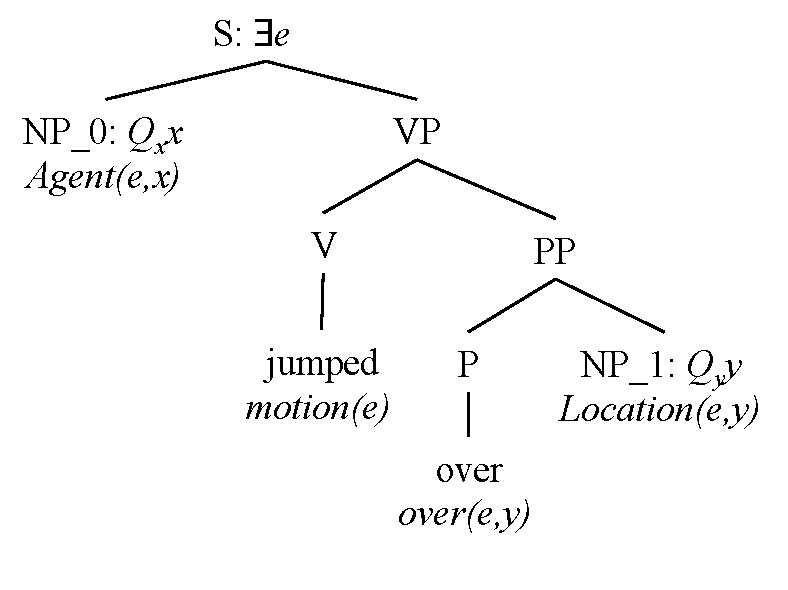
\includegraphics[width=.6 \linewidth ]{resources/ch5_resources/jump_declarative_semantics.pdf}
    \caption{XTAG declarative tree $\alpha$nx0Vpnx1 with associated semantics and variables}
    \label{fig:jump_declarative_semantics}
\end{centering}
\end{figure}

As with the semantic annotation work in \cite{sayeed2012incremental}, we introduce an extra ``quantification variable'' $Q$ for each entity/event variable in the semantic annotation. These variables can take on the value $\exists$ or $\forall$, representing the corresponding variable's quantification. Each quantification variable defaults to a value of $\exists$, but can have its value changed by specific determiners (such as ``every'') added through substitution/adjunction actions.

The declarative tree $\alpha$nx0Vpnx1 is shown with its subtree-associated VerbNet semantics in Figure \ref{fig:jump_declarative_semantics}. Semantics are shown in italics, and variables are shown following a colon for tree nodes which have them. We see that the $Agent$ and $Theme$ predicates, their associated free variables $x$ and $y$, and the associated variables' quantification variables $Q_x$ and $Q_y$ have been associated with the substitution nodes ``NP\_0'' and ``NP\_1'' respectively. The root node ``S'' is associated with the existentially quantified event variable $e$. The verbal anchor ``jumped'' adds the $motion$ predicate. The preposition ``over'' introduces the $over$ predicate. We can recover the full sentence semantics by traversing the tree and conjoining the semantics of each subtree.

\subsection{Increasing the semantic coverage of verb trees via metarules}

Each verb family in XTAG consists of a declarative tree and all of the valid syntactic transformations which it can undergo, shown in Table \ref{tab:metarules}. For example, starting from the transitive tree $\alpha$nx0Vnx1 (which would generate sentences such as ``the dog chased the cat''), we could apply a passive rule (``the cat was chased by the dog''), a dropby rule (``the cat was chased''), a relative clause extraction of the subject (``the dog that chased the cat''), and many others. Additionally, there are many valid combinations of these transformations such as a relative clause extraction of the object with a dropby (``the cat that was chased''). In total, there are 40 trees in the transitive family, including the declarative tree and its valid transformations.

In generating these syntactic transformations, we notice that the semantics undergo consistent transformations as well. When we apply a dropby rule (passive without by clause) to a tree, we have removed the semantics of the deleted argument node. From this intuition, we build a set of corresponding rules for how to alter the semantics under each syntactic transformation. Most of the semantic transformation is handled by the previous mapping of semantics to subtrees; when NP\_1 changes positions in the tree, it brings its associated variable and semantic annotations with it. The rules specify additional behavior for each transformation. We start with the most common transformations and leave the remaining rules as future work. The transformations we currently handle are as follows: passive, dropby, gerund, wh-subj, wh-sentsubj, wh-npobj, rel-adj-W, rel-adj-noW, rel-subj-W, rel-subj-noW, rel-subj-noW-forpassive, rel-obj-W, rel-obj-noW, PRO. These rules cover 37 of the 40 trees in the transitive family.

These transformations naturally fall into five groups, which we encode rules for separately. For each, we describe the semantic transformation, show an example tree, and give an example sentence it would be used in.
\begin{enumerate}
    \item \textbf{passives}: No additional semantic transformations necessary (when nodes are moved/deleted their semantics automatically follow). An example is shown in Figure \ref{fig:jump_passive_semantics}, which would be used to generate a sentence such as ``The river was jumped over''.

    \begin{figure}[H]
    \begin{centering}
    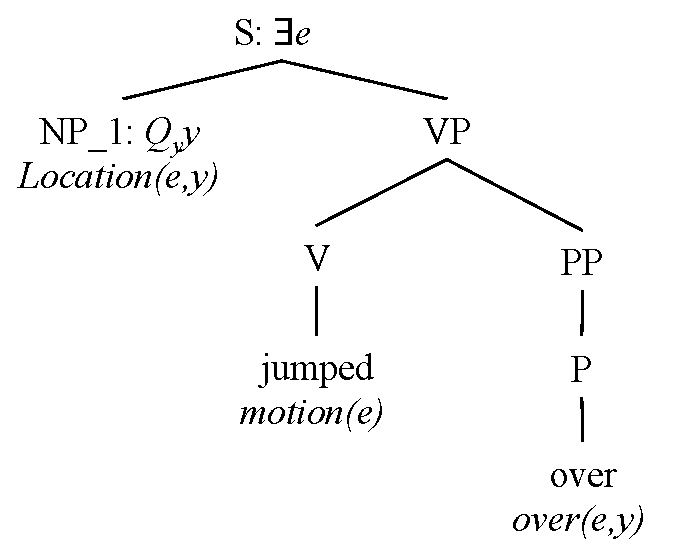
\includegraphics[width=.6 \linewidth ]{resources/ch5_resources/jump_passive_semantics.pdf}
    \caption{$\alpha$nx0Vpnx1 with dropby passive transformation of NP\_1 ($\alpha$nx1Vp)}
    \label{fig:jump_passive_semantics}
    \end{centering}
    \end{figure}

    \item \textbf{gerunds}: The new root node, which is an NP node, is annotated with the tree's event variable. An example is shown in Figure \ref{fig:jump_gerund_semantics}, which would be used for a sentence such as ``[The horse jumping over the river] scared the rider''.

    \begin{figure}[H]
    \begin{centering}
    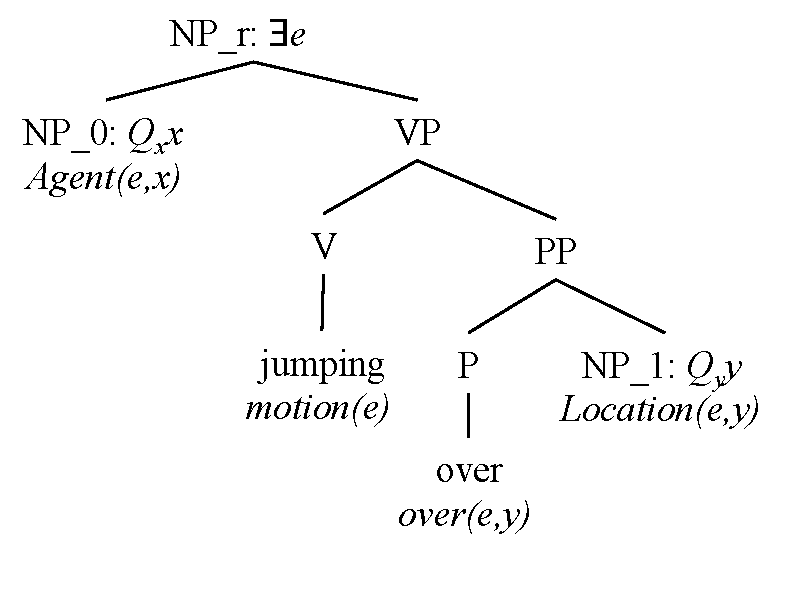
\includegraphics[width=.6 \linewidth ]{resources/ch5_resources/jump_gerund_semantics.pdf}
    \caption{$\alpha$nx0Vpnx1 with NP-gerund transformation ($\alpha$Gnx0Vpnx1)}
    \label{fig:jump_gerund_semantics}
    \end{centering}
    \end{figure}

    \item \textbf{wh-extractions}: The wh-extracted node is annotated with the entity variable from the original node. An example is shown in Figure \ref{fig:jump_wh_semantics} which would generate a sentence such as ``What did the horse jump over?''

    \begin{figure}[H]
    \begin{centering}
    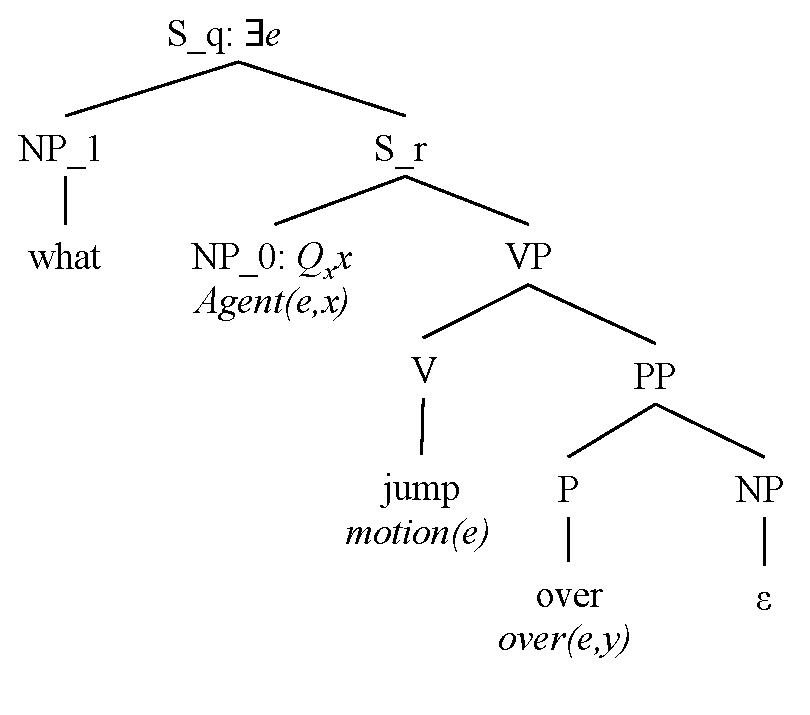
\includegraphics[width=.6 \linewidth ]{resources/ch5_resources/jump_wh_semantics.pdf}
    \caption{$\alpha$nx0Vpnx1 with wh-movement of NP\_1 ($\alpha$W1nx0Vpnx1)}
    \label{fig:jump_wh_semantics}
    \end{centering}
    \end{figure}

    \item \textbf{relative clauses}: The new root node, which is an NP or S node, is annotated with the entity/event variable of the extracted node. As example is shown in Figure \ref{fig:jump_relclause_semantics}, which would generate a sentence such as ``[The river which the horse jumped over] was a deep shade of blue''.

    \begin{figure}[H]
    \begin{centering}
    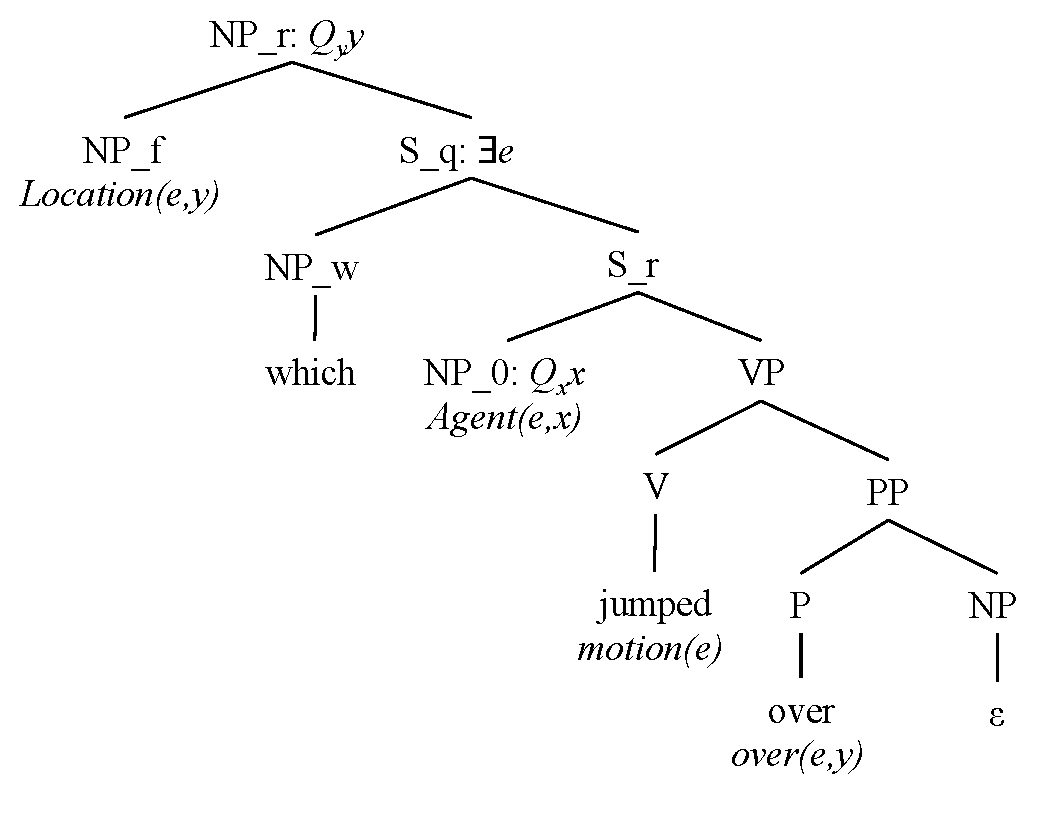
\includegraphics[width=.8 \linewidth ]{resources/ch5_resources/jump_relclause_semantics.pdf}
    \caption{$\alpha$nx0Vpnx1 with relative clause extraction of NP\_1 ($\beta$N1nx0Vpnx1)}
    \label{fig:jump_relclause_semantics}
    \end{centering}
    \end{figure}

    \item \textbf{PRO}: The semantics of the PRO node are deleted. An example is shown in Figure \ref{fig:jump_pro_semantics}, which would generate a sentence such as ``The horse likes [to jump over rivers]''.

    \begin{figure}[H]
    \begin{centering}
    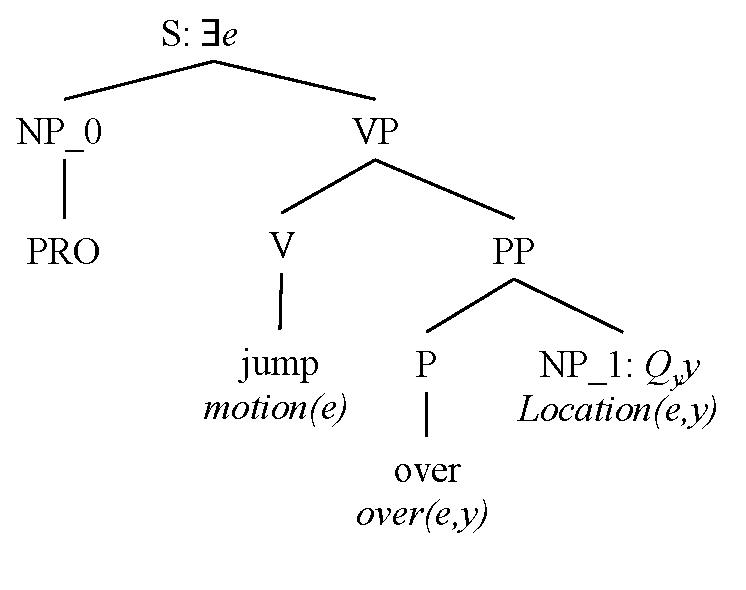
\includegraphics[width=.6 \linewidth ]{resources/ch5_resources/jump_pro_semantics.pdf}
    \caption{$\alpha$nx0Vpnx1 with PRO-subject transformation ($\alpha$nx0Vpnx1-PRO)}
    \label{fig:jump_pro_semantics}
    \end{centering}
    \end{figure}

\end{enumerate}

%As an example, Figure \ref{fig:jump_semantics_passive} shows the tree $\alpha$nx1Vp, which belongs to the same tree family as $\alpha$nx0Vpnx1, but has undergone a ``dropby'' diathesis alternation on the subject node, NP\_0. We would use this tree to generate a sentence such as ``the fence was jumped over.'' Looking at Figure \ref{fig:jump_semantics_passive}, we see that the dropby syntactic transformation automatically generated the corresponding tree semantics, as the semantic pieces were already mapped to subtrees.

The initial mapping of VerbNet roles to XTAG provided semantic annotations for
16 declarative trees (the remaining tree families that went unused were for idioms and small clauses).
With the application of semantic metarules, we have expanded the semantic coverage to 426 verbal subcategorization trees.

\pagebreak
\subsection{Composition Rules} 

\begin{figure}[h]
\begin{centering}
    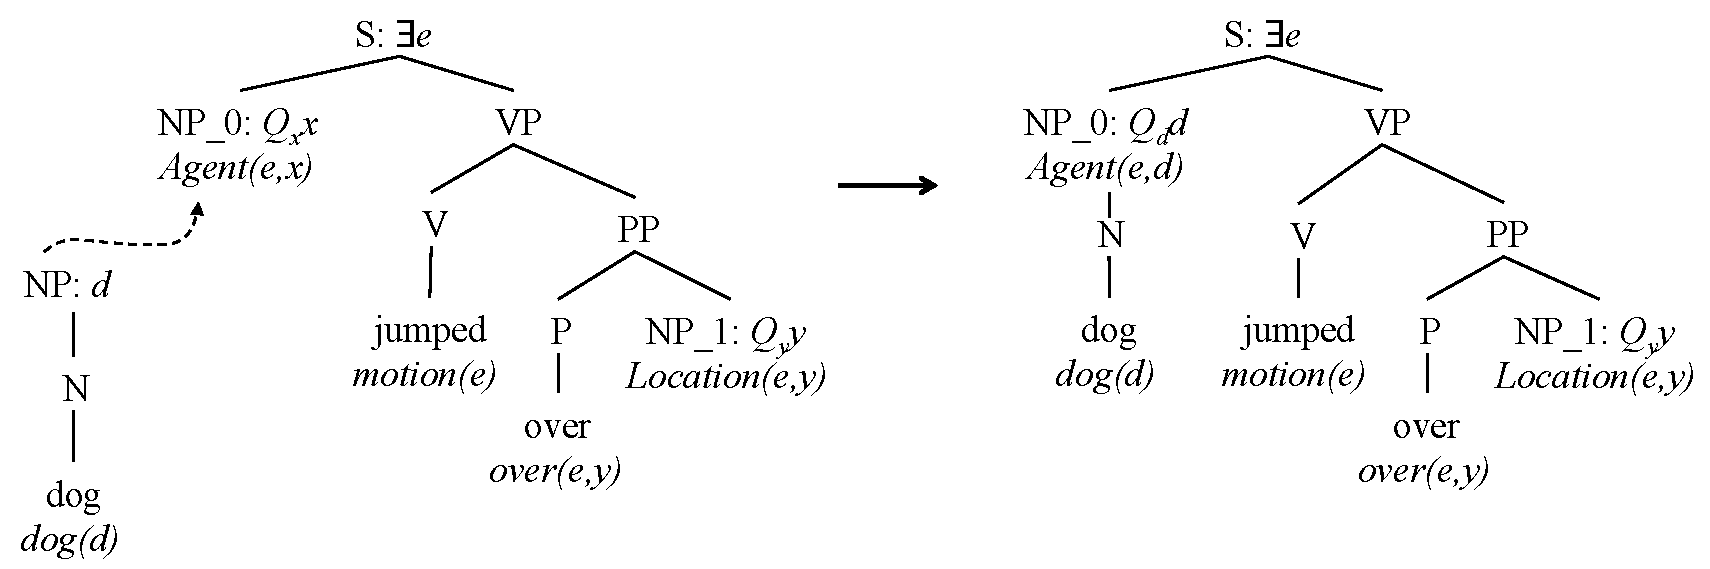
\includegraphics[width= \linewidth ]{resources/ch5_resources/neo_substitution.pdf}
    \caption{Example substitution in our grammar annotated with Neo-Davidsonian semantics}
    \label{fig:neo_substitution}
\end{centering}
\end{figure}

In associating semantic variables with subtrees, we have expanded the flexibility of our syntax/semantics interface, allowing us to greatly expand the semantic coverage via metarule application. However, we have deviated from the lambda notation used earlier; therefore, we must respecify the way in which elementary trees' semantics compose during substitution and adjunction. For substitution, we rebind the substitution node variable to the variable of the root of substituted elementary tree and conjunct the predicates. An example of this is shown in Figure \ref{fig:neo_substitution}. Here, $x$ gets bound to the variable $d$ introduced by the ``dog'' tree. Computing the full tree semantics, we now get $dog(d) \land Agent(e,d) \land motion(e) \land over(e,y) \land Location(e,y)$. 

\begin{figure}[h]
\begin{centering}
    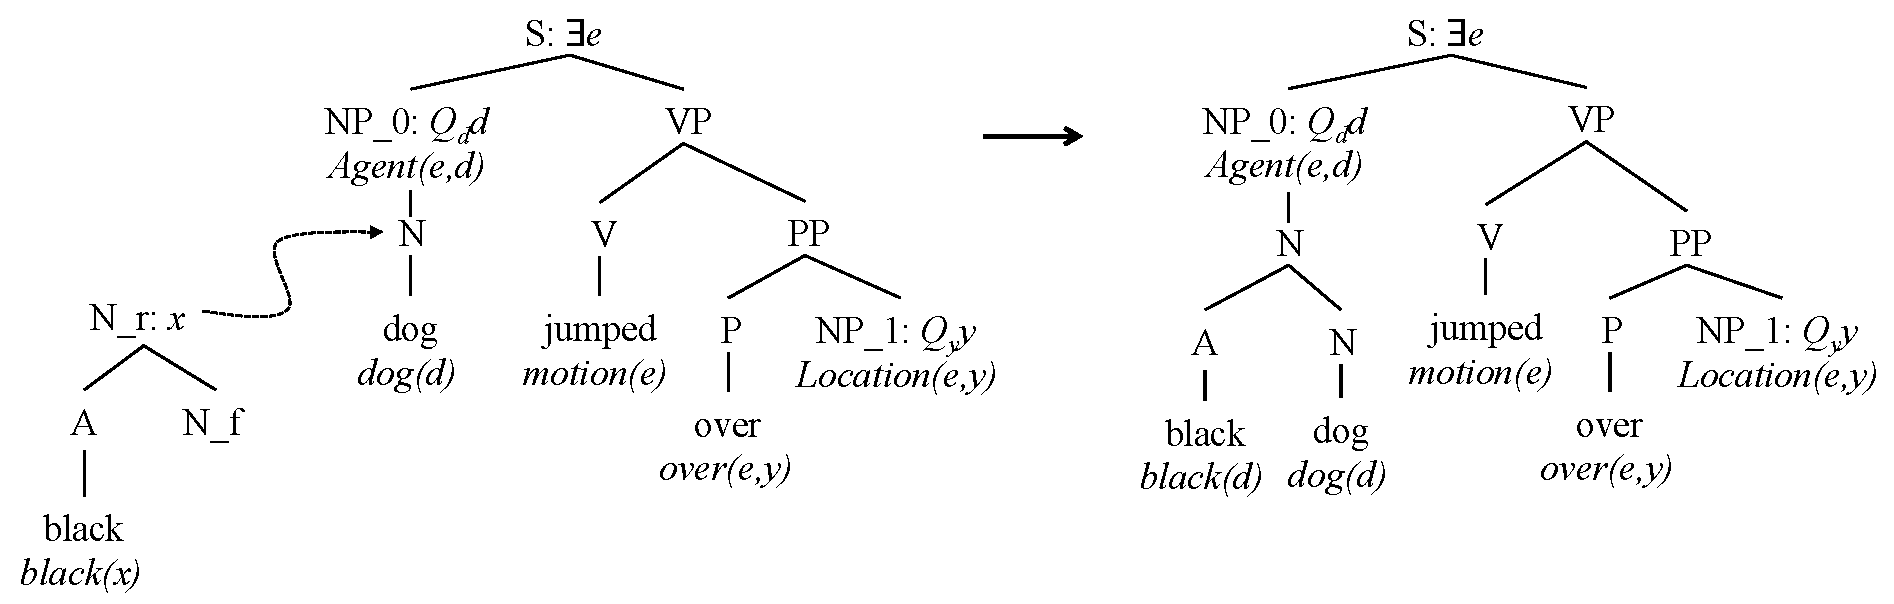
\includegraphics[width= \linewidth ]{resources/ch5_resources/neo_adjunction.pdf}
    \caption{Example adjunction in our grammar annotated with Neo-Davidsonian semantics}
    \label{fig:neo_adjunction}
\end{centering}
\end{figure}

For adjunction, we instead rebind the variable of the elementary auxiliary tree to the variable of the adjunction node, and then conjunct the predicates. If a node does not have an associated variable, we take the variable the shortest distance above it in the tree, as in the semantic work done in \cite{sayeed2012incremental}. For example, the variable for the $N$ node in Figure \ref{fig:neo_substitution} is $d$, coming from the ``NP\_0'' node above it. An example of adjunction is shown in Figure \ref{fig:neo_adjunction}, where the ``black'' tree adjoins onto the noun whose child is ``dog''. The ``N'' node's variable $d$ gets bound to the auxiliary trees variable $x$. This results in the final semantics of $black(d) \land dog(d) \land Agent(e,d) \land motion(e) \land over(e,y) \land Location(e,y)$. 

\begin{figure}[h]
\begin{centering}
    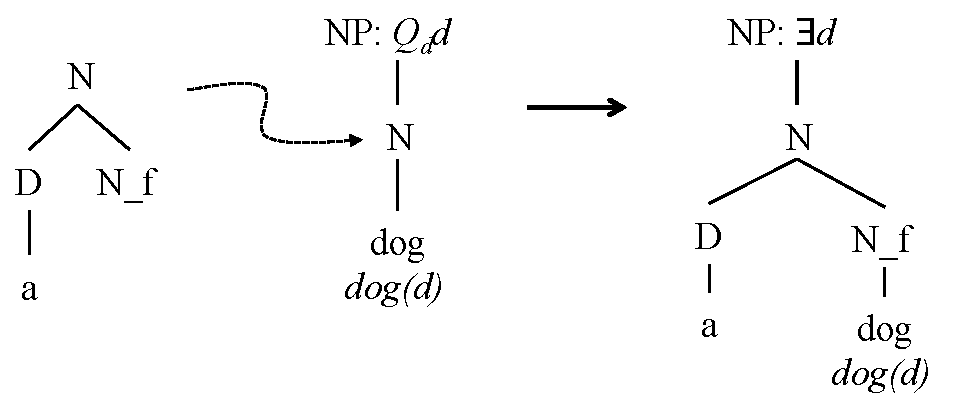
\includegraphics[width=.6\linewidth ]{resources/ch5_resources/neo_existential.pdf}
    \caption{Example of determiner adjunction adding explicit existential quantification}
    \label{fig:neo_existential}
\end{centering}
\end{figure}

The final consideration during composition is replacing our $Q$ variables when determiner actions are applied. For mass nouns which do not require determiners, (such as ``dogs'' in the sentence ``dogs chase cats''), the quantification is assumed to be universal. Otherwise, when a determiner is applied it replaces the $Q$ variable with either $\exists$ or $\forall$. An example of existential quantification is shown in Figure \ref{fig:neo_existential}. $Q_d$, the quantification for $d$, is explicitly set to $\exists$. A similar procedure occurs for universal quantification, as shown in Figure \ref{fig:neo_universal}. However in the case of universal quantification, computing the full tree semantics requires an implication. Choosing the correct position for the implication could be done by analyzing the structure of the derived tree; however, the semantic research in \cite{sayeed2012incremental} argues that we can use the semantic expressions themselves to determine the position. They argue that the lack of an event variable is a cue for the implication position, as everything containing the event variable is part of what is implied by the universal quantification. Traversing the tree in Figure \ref{fig:neo_universal}, the first predicate following the universal quantification that does not have $e$ as an argument is $dog(d)$. Therefore, our full semantic expression for this tree is $\forall d, dog(d) \rightarrow Agent(e,d) \land motion(e) \land over(e,y) \land Location(y)$.

\begin{figure}[h]
\begin{centering}
    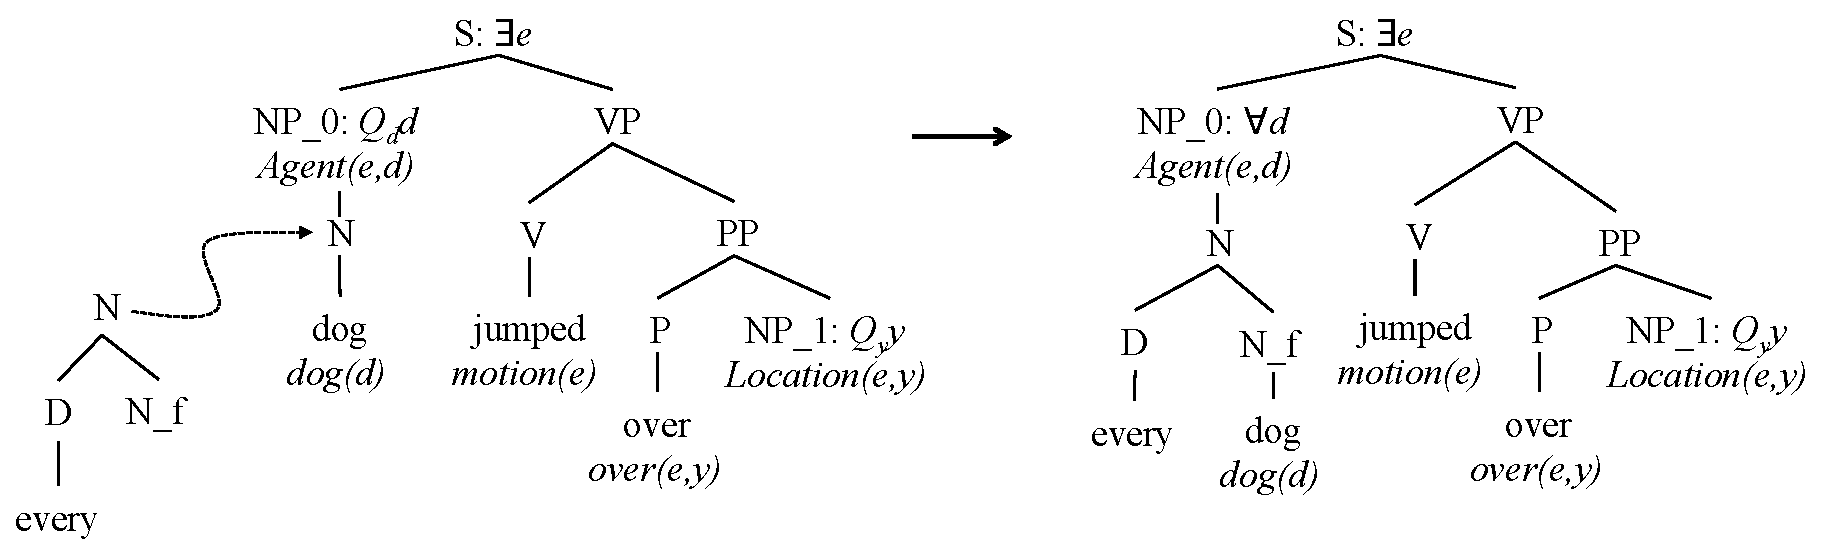
\includegraphics[width= \linewidth ]{resources/ch5_resources/neo_universal.pdf}
    \caption{Example of determiner adjunction adding universal quantification}
    \label{fig:neo_universal}
\end{centering}
\end{figure}

\section{Evaluating the Grammar Coverage}

\begin{figure*}[h]
    \centering
    \begin{subfigure}{0.6\textwidth}
        \centering
        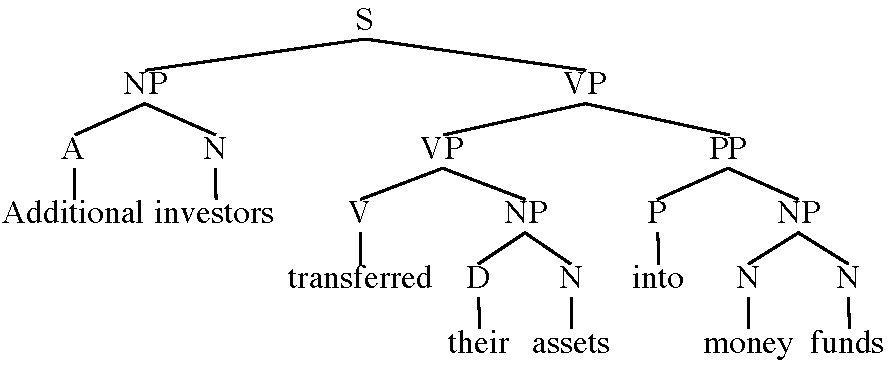
\includegraphics[width=1.0 \linewidth ]{resources/ch5_resources/parse_example.pdf}
        \caption{Parse Tree}
        \hfill
        \hfill
    \end{subfigure}
    \begin{subfigure}{0.6\textwidth}
        \centering
        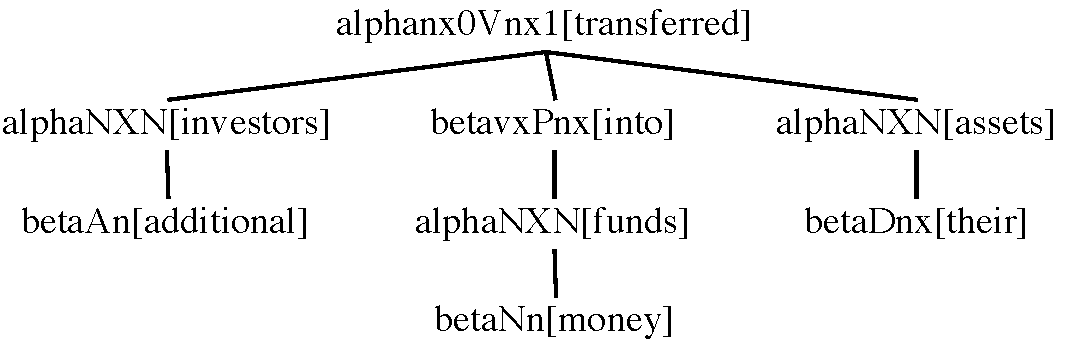
\includegraphics[width=1.0 \linewidth ]{resources/ch5_resources/deriv_example.pdf}
        \caption{Derivation Tree}
    \end{subfigure}
    \begin{subfigure}{0.3\textwidth}
        \centering
        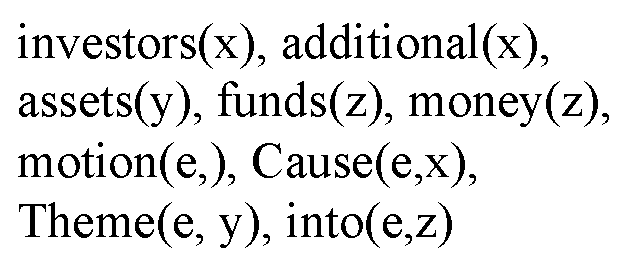
\includegraphics[width=1.0 \linewidth ]{resources/ch5_resources/derivation_semantics.pdf}
        \caption{Computed Semantics}
    \end{subfigure}
    \centering
    \caption{Example parse and computed Neo-Davidsonian semantics for WSJ sentence}
    \label{fig:neo_wsj_example}
\end{figure*}

At this point, we now have a grammar with substantially wider coverage and higher quality semantics than the grammar we introduced previously for the S-STRUCT experiments. We now revisit the section of the WSJ corpus that has LTAG parses to show the utility of this new grammar. Revisiting the example parse shown in Figure \ref{fig:wsj_example}, we re-derive the semantics with the Neo-Davidsonian annotated grammar, resulting in the semantic annotation shown in Figure \ref{fig:neo_wsj_example}. In this semantic representation, rather than just have a $transfer$ predicate, we have $motion$, $Cause$, and $Theme$ predicates, telling us that the assets were moved to a money fund on the volition of the investors. This demonstrates the higher quality abstractions captured by the VerbNet semantics.

In the S-STRUCT dataset, there were $18159$ WSJ sentences that were successfully parsed by the LTAG parser. Of these, the previous grammar successfully derived semantics for $7500$ ($41\%$). Our new grammar, with the larger set of semantically annotated verb subcategorization trees, successfully derives semantics for $14708$ of these ($81\%$). 

\subsection{Extending the LTAG Parser}

\begin{figure}[h]
\begin{centering}
    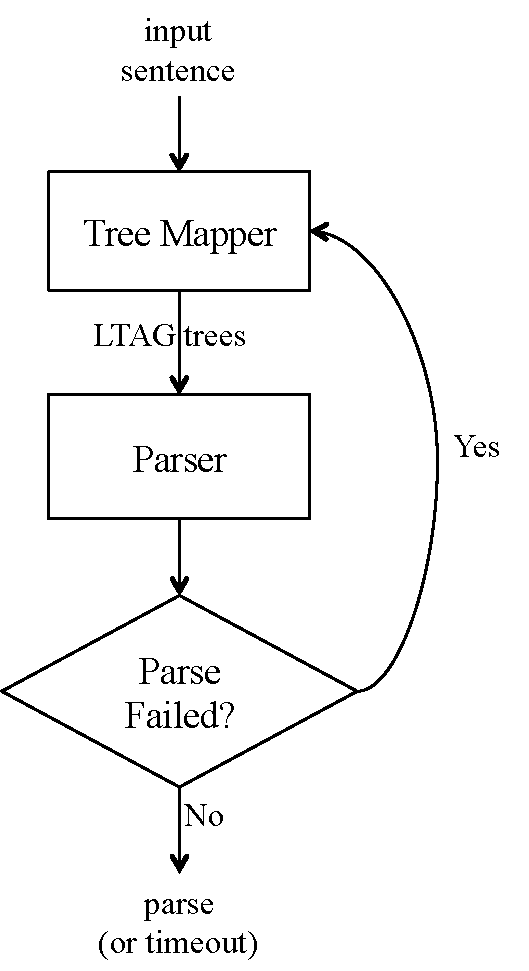
\includegraphics[width= 0.4\linewidth ]{resources/ch5_resources/tree_mapper_diagram.pdf}
    \caption{Diagram of LTAG parser with tree mapper feedback}
    \label{fig:tree_mapper_diagram}
\end{centering}
\end{figure}

One major source of data loss in the grammar evaluation is the LTAG parser; many sentences in the WSJ do not return a parse, either because none are found, or the parser times out. In this section, we modify the LTAG parser in order to capture more of the WSJ dataset that was not previously parsable. One reason the parser fails is the preprocessing step of mapping input words to lexicalized trees. If trees are missing from this mapping procedure, a valid parse may not exist; if there are too many trees, the parser will timeout. To solve this, we replace the standard parsing pipeline with the feedback loop shown in Figure \ref{fig:tree_mapper_diagram} which allows us to start with a small set of trees and repeatedly add to this set until either a parse is found or the parser times out. To choose the best parse from the set of parses returned, we minimize the PARSEVAL bracket-crossing against the gold-standard, as in Section \ref{sec:sstruct_dataset} \cite{parseval}.

Using this new parsing architecture, we increase the number of parsable WSJ sentences to $26038$. Of these, our grammar successfully derives semantics for $19266$ ($74\%$), showing the wide-coverage of this grammar. The remaining $26\%$ could be recovered by adding semantic annotations for additional ``individual trees'', which remains as future work.

% include your own bib file like this:
%\bibliographystyle{acl}
%\bibliography{acl2017}
\bibliography{acl2017}
\bibliographystyle{acl_natbib}

\end{document}
